\chapter{Extending the $\mu$ Control Sample to a Signal Sample}
\label{ch:ra4}

In Chapter~\ref{ch:ra1}, the muon control sample was used to predict the background contribution from W and \tto events. The muon likelihood's incorporation into the overall likelihood in order to interpret the hadronic results allowed for some small signal contamination. However it was in general viewed as a constraint on the ``signal" region of the hadronic selection. 

The selection outlined in Section~\ref{sec:muon} was designed to select events from Standard Model W decays, hence minimising the contamination from signal. However, as the simultaneous fit includes the signal efficiency in the $\mu$ control sample it is possible to relax the cuts and allow more potential signal into the $\mu$ yield. Instead of viewing it as a control sample it may then be considered as a second signal sample in the simultaneous fit. The electroweak background behaviour is still constrained by the flat behaviour in \RaT whereas the presence of signal would exhibit an exponentially increasing behaviour. Thus it is possible to construct a dual-sample search in order to extend the reach of the analysis.  The following work represents the author's personal investigation into the effect of increasing the chance for signal contamination in the $\mu$ selection on the eventual limit with the current dataset. 

\subsection{Relaxing the Cuts}

The primary cut in the $\mu$ control sample responsible for restricting the signal is the M$_{T}$ requirement, as it puts a restriction on boosted W decays. The first step is to remove this cut, allowing more potential signal into the sample. Having done so there are three possible scenarios with respect to the \alt cut. Using the \alt cut as defined in the hadronic analysis is a natural choice. However the use of an \alt cut limits the statistics, so removing this cut would increase the muons sample statistics. Conversely, using the hadronic definition of the \alt cut where the muon is not considered leads to the false appearance of missing energy, hence allowing more background into the sample. The use of the leptonic version of \alt, $\alpha^{lep}_{T}$ cut as defined in Section~\ref{sec:lalt} does not suffer from this issue, but as this is a tighter cut will reduce the available statistics. 

The four $\mu$ selection criteria considered are therefore:

\begin{itemize}
\item 2011 Selection (unchanged)
\item a) No M$_{T}$ Cut and use the \alt $> 0.55$ cut from the hadronic analysis where the muon is ignored (as previously in the 2011 selection)
\item b) No M$_{T}$ Cut and take out the \alt cut (the $\sfrac{\MHT}{\HT} >$ 0.4 cut ensures the elimination of QCD background is maintained)
\item c) No M$_{T}$ Cut and make a cut with the leptonic \alt, $\alpha^{lep}_{T}$ $>$ 0.55
\end{itemize}

The one muon requirement cut and the other cuts mentioned in Section~\ref{sec:muon} remain as they do not pertain to the rejection of signal but rather the selection of a good isolated muon not overlapping with a jet, in the case where the decay is not from a Z where a second $\mu$ is not identified by the quality criteria. The $\sfrac{\MHT}{\HT}$ cut is generally superseded by the \alt cut therefore removing it has little effect, however it is left in so that in the case where the \alt cut is removed we remain in the kinematic phase space of the hadronic signal region. 

\subsection{Event Yields}

The bin-by-bin yields in Monte Carlo normalised to 1.1fb$^{-1}$ for the Standard Model backgrounds (B) and potential signal (S) from LM6 are shown in Table~\ref{tab:ra4a}. The values of the ratio $\sfrac{S}{\sqrt{B}}$ are also shown as a measure of the potential significance of LM6 signal in each bin. As in the hadronic selection, where signal is present it shows the greatest significance with regards to background in the highest \HT bins. Removing the M$_{T}$ cut raises the ratio \srb in the highest three bins whilst in the lower bins \srb has fallen due to the increase of background. As expected removing the \alt cut lowers the \srb as more background enters the selection, but the available statistics are higher. In the case where the muon is used in the \alt definition the ratio is improved in all bins. The values in the highest two bins are large but currently suffer from low available Monte Carlo statistics in the SM backgrounds. 

\begin{table}[htbp]
\centering
\footnotesize
\begin{tabular*}{0.99\linewidth}{@{\extracolsep{\fill}}c c c c c c}
\hline
\hline
& \scalht Bin (GeV) & 275--325 & 325--375 & 375--475 & 475--575 \\ [0.5ex]
\hline
\hline
\multirow{3}{*}{2011 Selection} & B (SM) &407.5 & 179.1  & 131.6 & 48.7 \\
&S (LM6)&0.15 & 0.15 & 0.53 & 0.82\\
& $\sfrac{S}{\sqrt{B}}$ & 0.000 & 0.001 & 0.004 & 0.017\\
\hline
\multirow{3}{*}{a) No M$_{T}$ Cut \& \alt $>$ 0.55} & B (SM) &549.93 &243.33&179.51 &63.80 \\
&S (LM6)& 0.19 & 0.20 & 0.59 & 0.92 \\& $\sfrac{S}{\sqrt{B}}$  & 0.000 & 0.001 & 0.003 & 0.0014 \\
\hline
\multirow{3}{*}{b) No M$_{T}$ Cut \& No \alt} & B (SM) &1335.81& 603.61 & 485.62 & 192.61\\
&S (LM6) &0.26&0.32&0.89&1.43\\
& $\sfrac{S}{\sqrt{B}}$  & 0.000 & 0.001 & 0.002 & 0.007 \\
\hline
\multirow{3}{*}{c) No M$_{T}$ Cut \& \alt$_{lep}$ $>$ 0.55} & B (SM) & 163.95 & 70.64 & 39.87  & 16.38  \\
& S (LM6) & 0.13 & 0.17 & 0.51 & 0.79 \\
& $\sfrac{S}{\sqrt{B}}$ & 0.001 & 0.002 & 0.013 & 0.048 \\
\hline
\hline
\end{tabular*}
\newline
\newline
\newline
\begin{tabular*}{0.99\linewidth}{@{\extracolsep{\fill}}c c c c c c}
\hline
\hline
& \scalht Bin (GeV) & 575--675 & 675--775 & 775--875 & 875--$\infty$  \\ [0.5ex]
\hline
\hline

\multirow{3}{*}{2011 Selection} & B (SM) &13.32  & 7.95  & 3.20 & 0.97 \\
&S (LM6)&1.09 & 1.17 & 0.95 & 1.21\\
& $\sfrac{S}{\sqrt{B}}$  & 0.082 & 0.147 & 0.297 & 1.343\\
\hline
\multirow{3}{*}{a) No M$_{T}$ Cut \& \alt $>$ 0.55} & B (SM) & 18.53 & 8.59 & 3.34 & 0.97 \\
&S (LM6)& 1.23 & 1.35 & 1.08 & 1.42 \\
& $\sfrac{S}{\sqrt{B}}$ & 0.066 & 0.157 & 0.324 & 1.5747 \\
\hline

\multirow{3}{*}{b) No M$_{T}$ Cut \& No \alt} & B (SM) & 67.64 & 30.04 & 12.77 & 3.26 \\
&S (LM6) &1.87 & 2.04 & 1.77 & 3.07\\
& $\sfrac{S}{\sqrt{B}}$  & 0.028 & 0.068 & 0.139 & 0.940 \\
\hline
\multirow{3}{*}{c) No M$_{T}$ Cut \& \alt$_{lep}$ $>$ 0.55} & B (SM) & 7.85 & 1.76 & 0.05 & 0.05  \\
& S (LM6) & 1.05 & 1.13 & 0.89 & 1.06 \\
& $\sfrac{S}{\sqrt{B}}$  & 0.134 & 0.641 & 19.282 & 22.982 \\
\hline
\hline
\end{tabular*}

\caption{\label{tab:ra4a}Monte Carlo yields for $\mu$ control sample for Standard Model Monte Carlo (B) and potential SUSY signal from test point LM6. Four separate selection criteria are considered:  2011 Selection as detailed in Chapter ~\ref{ch:ra1} alongside three selections with the M$_{T}$ cut removed and different approaches to the \alt cut: a) \alt $>$ 0.55, b) \alt cut removed and c) \alt$^{lep}$ $>$ 0.55 as detailed in Section~\ref{sec:lalt}}
\end{table}

The ratio \srb can be further explored in the $m_{0}-m_{1/2}$ plane of the CMSSM using the SUSY Signal Scan used previously to set exclusion limits. Figure~\ref{fig:4sb} shows the values of \srb for 1.1fb$^{-1}$ across the region relevant to the exclusion limit, using the four highest bins only (\HT $>$ 575). These bins are chosen as an illustration of the effect of the different criteria on the sensitivity of the muon signal sample, although the eventual fit is an \HT shape analysis and therefore is affected by the shape of \srb across all bins. Across the full range of SUSY points the conclusions fit those identified in the table for LM6, although the criteria a) and b) with the M$_{T}$ cut removed show little difference from the previous 2011 selection, in terms of increasing the number of signal points that reach a certain \srb at this luminosity. On the other hand, the use of the leptonic cut \altl \more 0.55 shows a noticeable increase in the number of points achieving a certain \srb. 



\begin{figure}[htbp]
\centering
\subfigure[]{\includegraphics[width=0.49\textwidth]{Figures/RA4/SoversqrtB_AsWas.pdf}}
\subfigure[]{\includegraphics[width=0.49\textwidth]{Figures/RA4/SoversqrtB_noMT_hat.pdf}}
\subfigure[]{\includegraphics[width=0.49\textwidth]{Figures/RA4/SoversqrtB_noMT_noat.pdf}}
\subfigure[]{\includegraphics[width=0.49\textwidth]{Figures/RA4/SoversqrtB_noMT_lat.pdf}}
\caption{\label{fig:4sb}The signal to background ratio $\srb$ for each point in the CMSSM ($m_{0},m_{1/2}$) plane for the four different $\mu$ selection criteria at NLO cross sections for events \HT $>$ 575 (the four highest bins). The 2011 Selection (a) is unchanged from Chapter~\ref{ch:ra1}. The M$_{T}$ cut is removed for (a) with \alt $>$ 0.55, (b) with no \alt cut and (c) with $\alpha^{lep}_{T}$ $>$ 0.55.}
\end{figure}





\subsection{Fit Results}

The event yields from the previous section are then entered into the simultaneous likelihood fit described previously in Section~\ref{sec:fit}. The presence of signal in both the hadronic selection and the muon selection is allowed and the hadronic and photon sample results are unchanged from the 2011 analysis. The CL$_{s}$ value is again calculated in the $m_{0}-m_{1/2}$ plane for each of the four selection definitions. The results of the test (CL$_{s}$ \more 0.05) are shown in Figure~\ref{fig:4fit}, where those points for which this is true are shown red, corresponding to a 95\% confidence in excluding that point. Points for which the test is false are shown blue, and points missing due to insufficient Monte-Carlo statistics are not plotted. 



\begin{figure}[htbp]
\centering
\subfigure[]{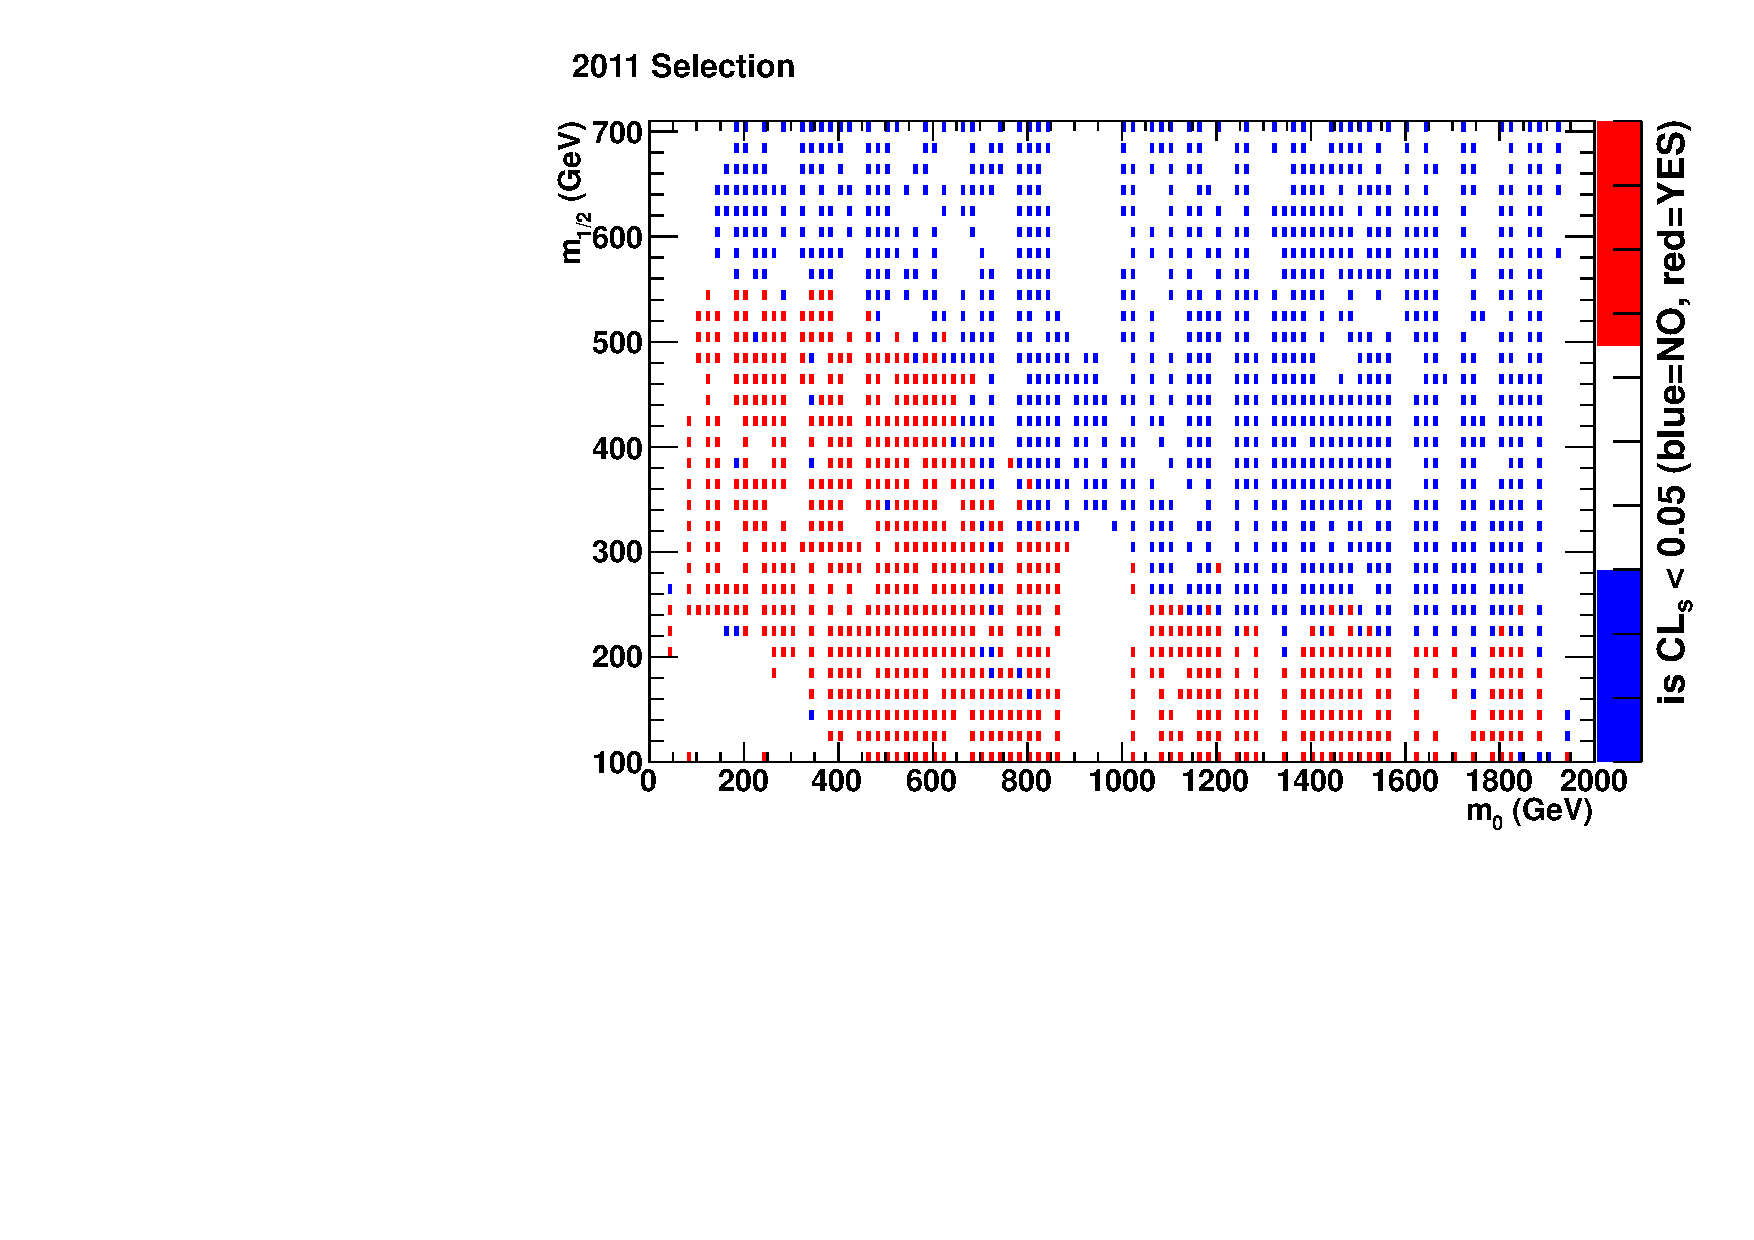
\includegraphics[width=0.49\textwidth]{Figures/RA4/AsWas_Modified_CLs}}
\subfigure[]{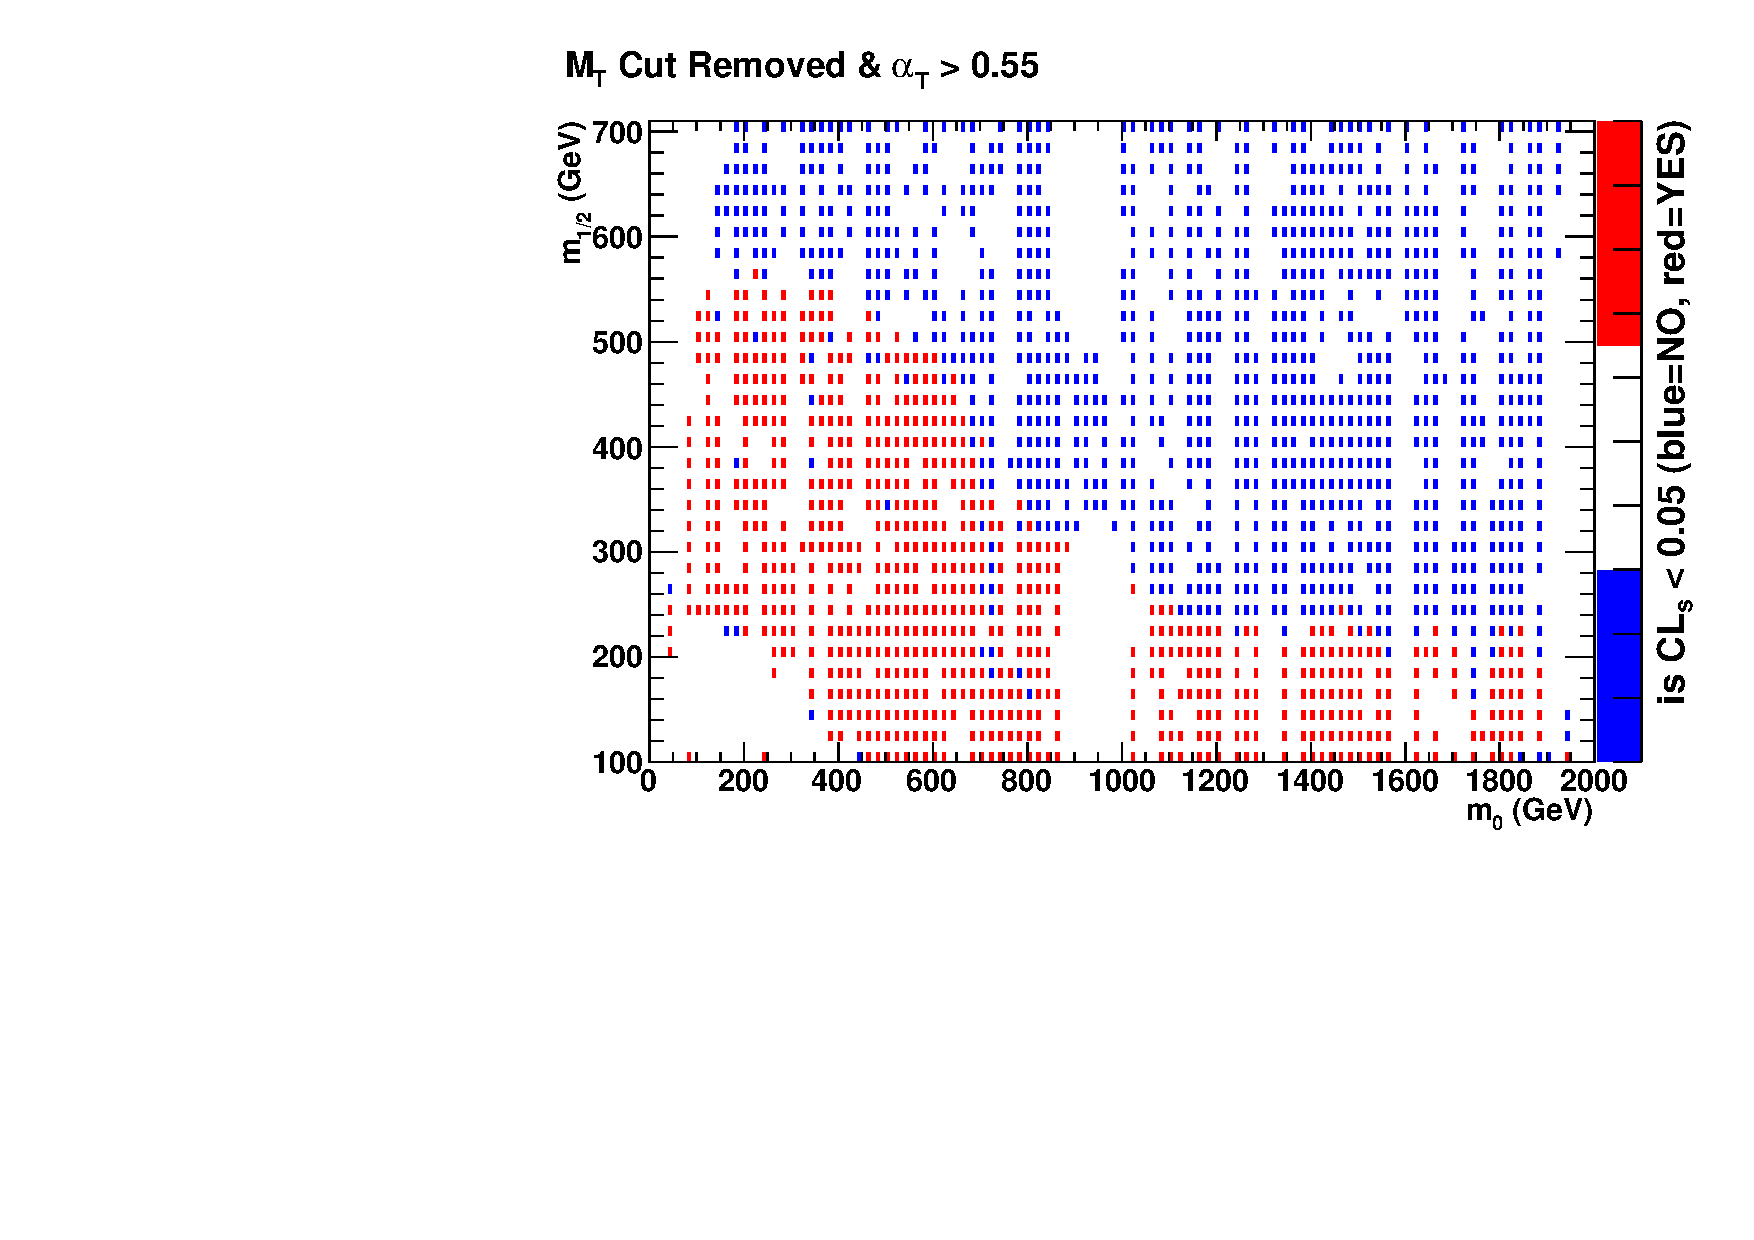
\includegraphics[width=0.49\textwidth]{Figures/RA4/hat_Modified_CLs}}
\subfigure[]{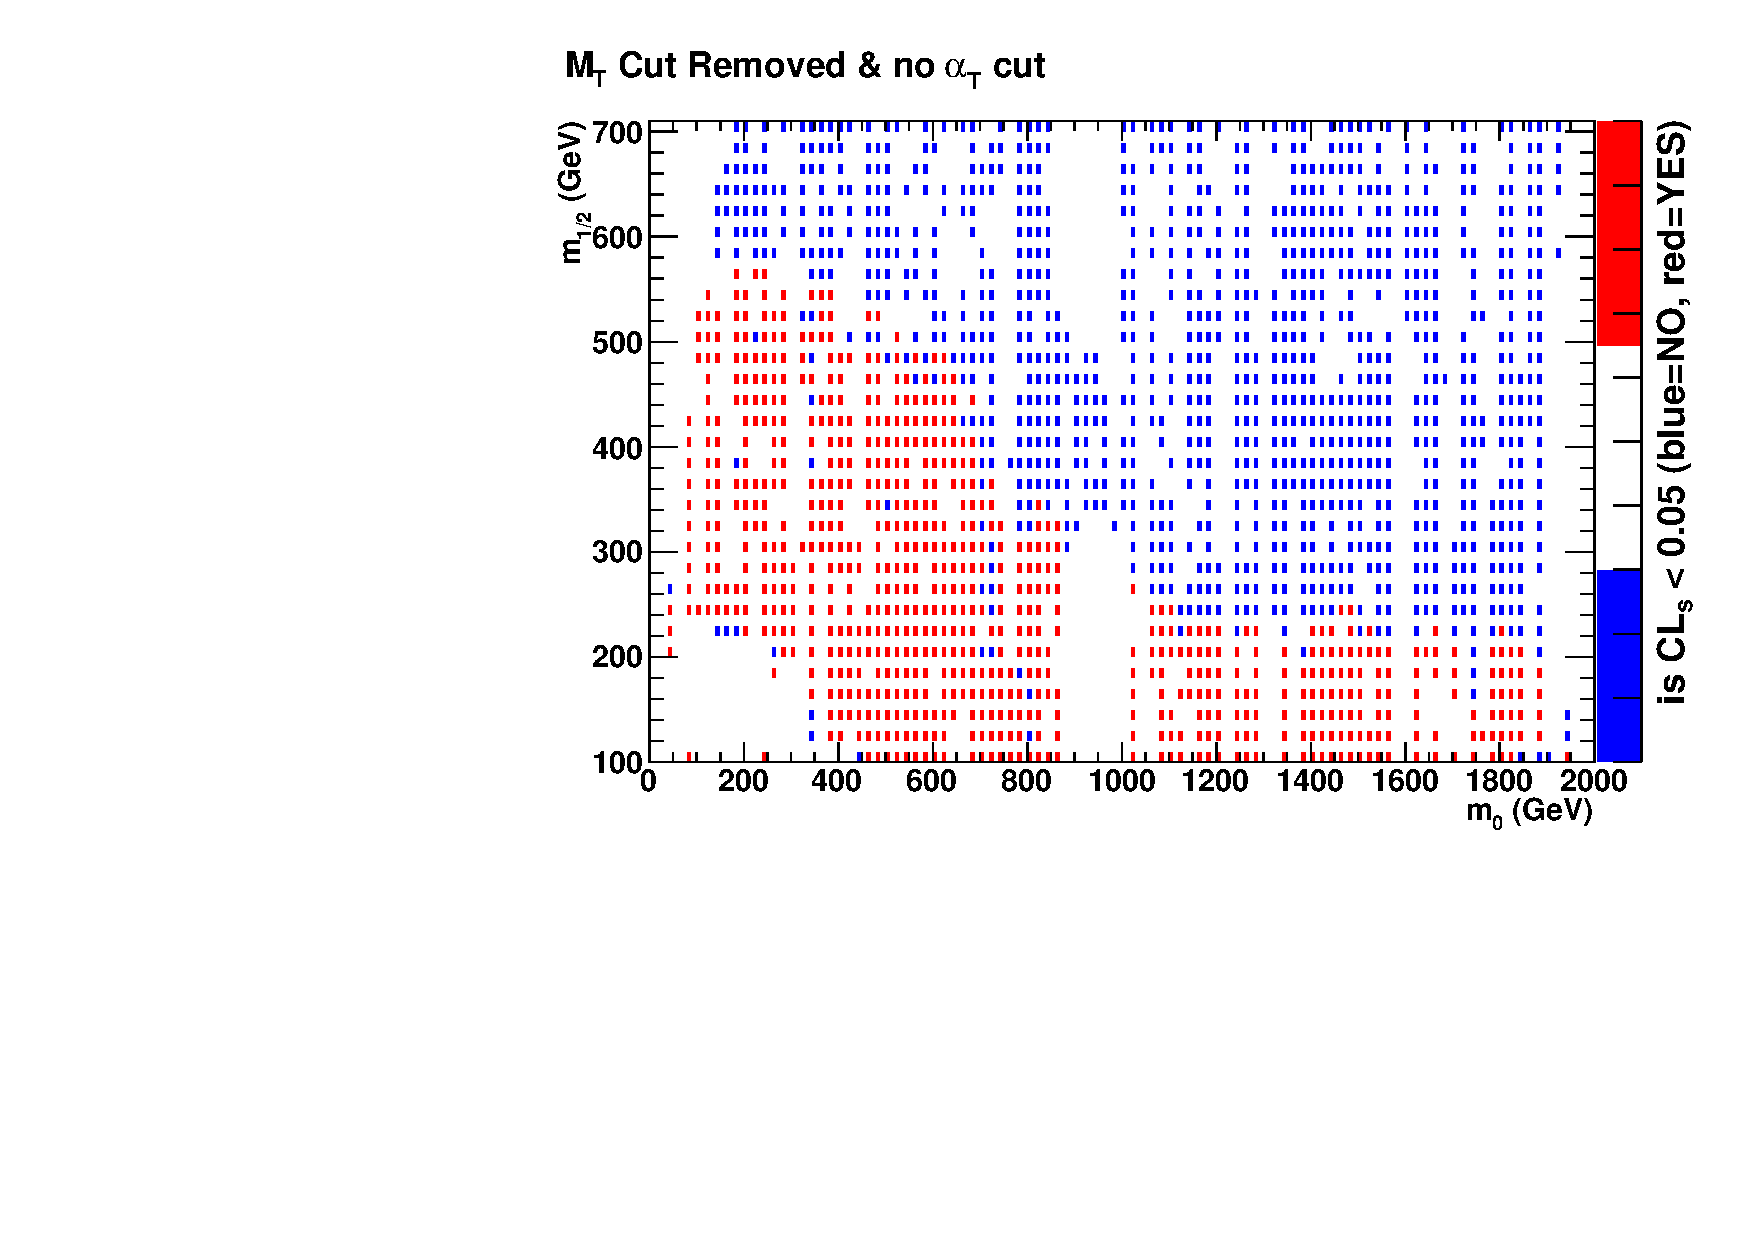
\includegraphics[width=0.49\textwidth]{Figures/RA4/noat_Modified_CLs}}
\subfigure[]{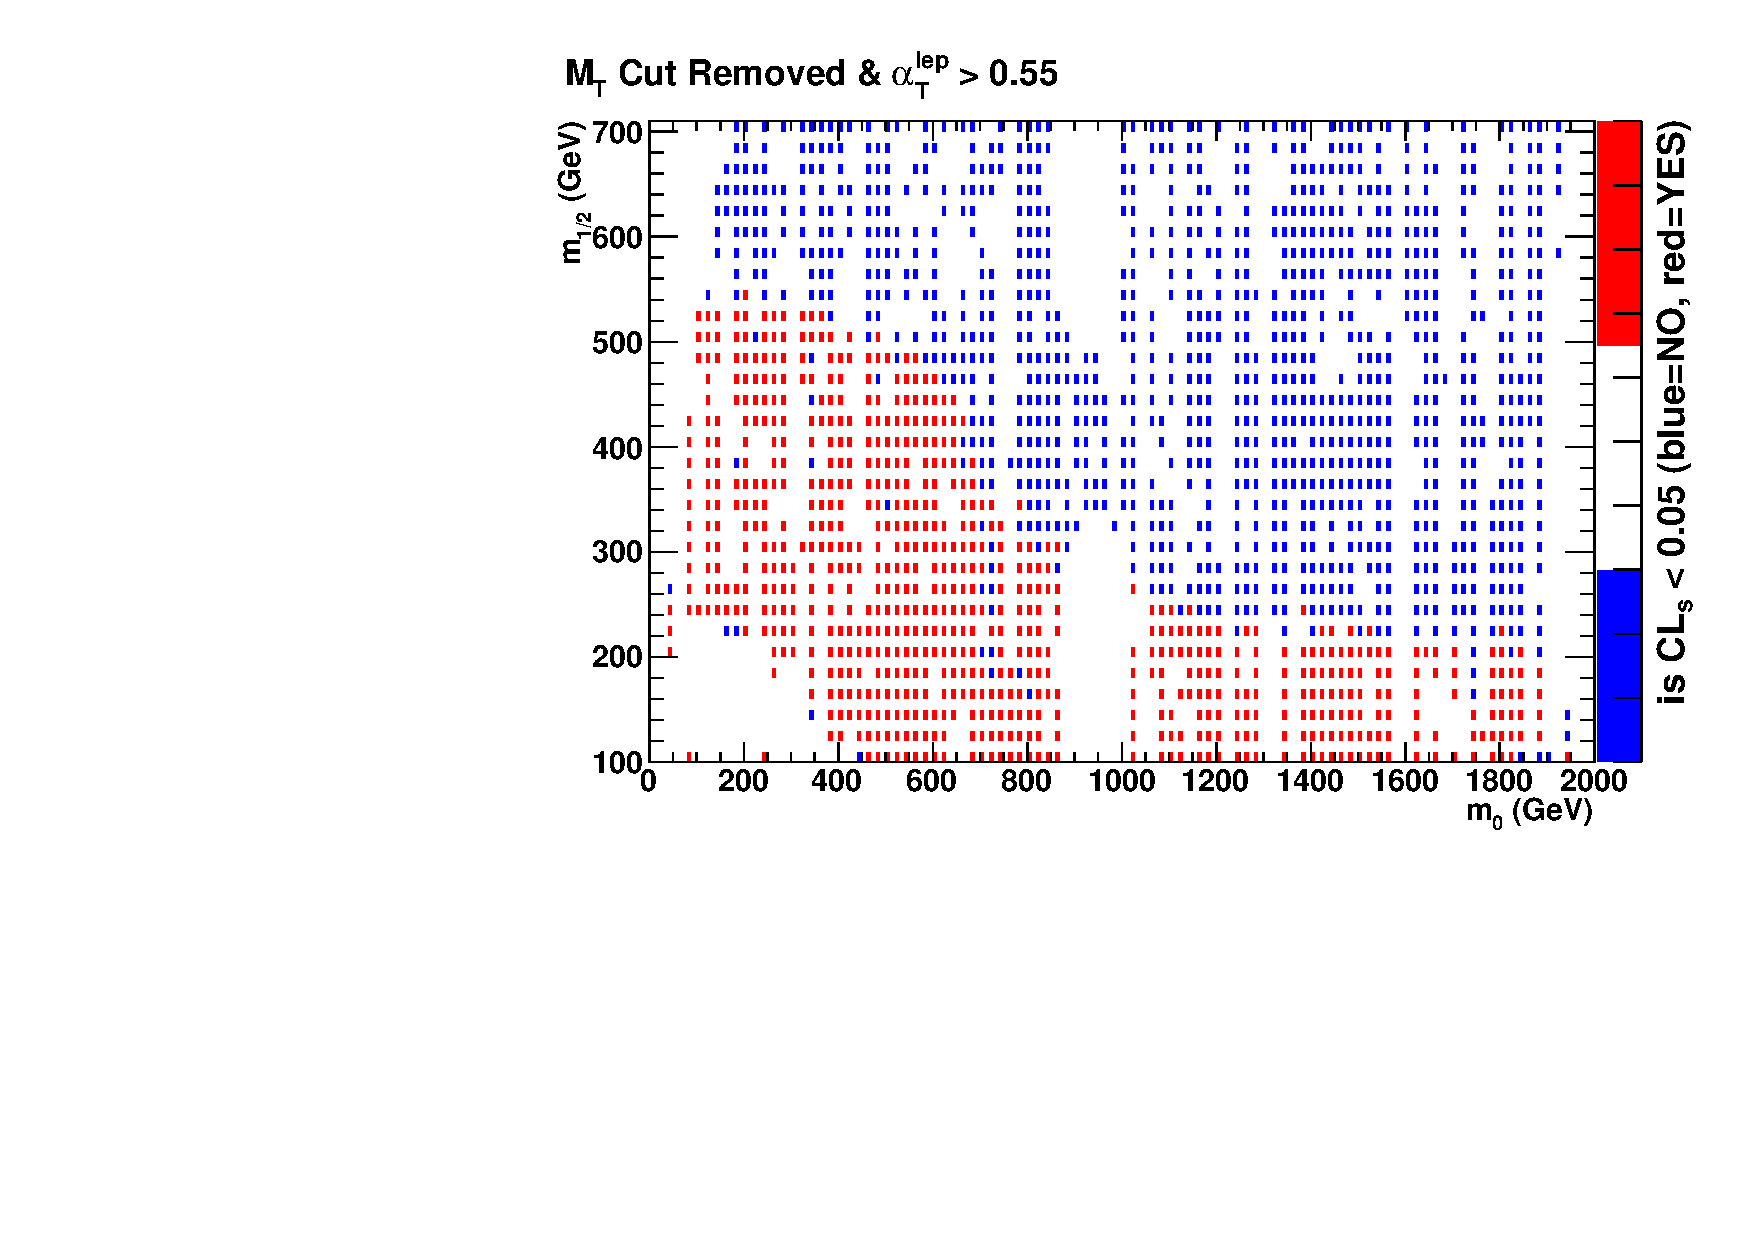
\includegraphics[width=0.49\textwidth]{Figures/RA4/lat_Modified_CLs}}
\caption{\label{fig:4fit}The CL$_{s}$ exclusion limit for the four different $\mu$ selection criteria, with CL$_{s}$ $<$ 0.05 shown in red (excluded at 95\% confidence) and CL$_{s}$ $>$ 0.05 shown in blue. Not all points were calculated due to a lack of sufficient MC data. The 2011 Selection (a) is unchanged from Chapter~\ref{ch:ra1} and corresponds to the final limit plot there. The M$_{T}$ cut is removed for (a) with \alt $>$ 0.55, (b) with no \alt cut and (c) with \alt$^{lep}$ $>$ 0.55.}
\end{figure}



The results of the fit show no marked difference in the eventual result between the four categories. In the extreme low m$_{0}$ region where the reach in m$_{1/2}$ is greatest, the criteria which extends the limit slightly with respect to the 2011 analysis is the removal of the alpha$_{T}$ cut, indicating the additional statistics slightly improve the limit, although the difference is slight. The lowered statistics of the leptonic \altl cut does not affect the exclusion power. 

\section{Interpretation}

At this luminosity the CL$_{s}$ exclusion power of the likelihood fit shows no significant change of power with the removal of the $M_{T}$. Therefore it is safe to remove the M$_{T}$ cut in future iterations of this analysis and allow more signal into the $\mu$ sample.  The limited statistics found by the selection requiring the leptonic \alt cut does not affect the exclusion power over the hadronic cut, or removal entirely. In addition the use of this cut significantly increases the significance, \srb, in the higher bins of \HT indicating a large impact in the shape analysis. As moving to higher luminosities will increase both the statistics available using this definition and the potential \srb, this definition is suitable for defining a $\mu$ signal sample for used in a dual-signal search strategy alongside the hadronic signal selection. Although this provides no greater limit at the present luminosity it is recommended to investigate further in the next luminosity update.


